%!TEX root=kinneer_seke.tex
% mainfile: kinneer_seke.tex

\documentclass[hyperref]{beamer}
% \includeonlyframes{current}

\usecolortheme[accent=blue,dark]{solarized}

\beamertemplatetransparentcovered

\usepackage[utf8]{inputenc}
\usepackage{merriweather}
\usepackage{moresize}
\usepackage{anyfontsize}
\usepackage{xcolor}
\usepackage{graphicx}

\usepackage{pgfplots}
\pgfplotsset{compat=1.9}
\usepgfplotslibrary{colormaps,external}

\usepackage{pifont}
\newcommand{\cmark}{{\color{solarizedGreen}\ding{51}}}
\newcommand{\xmark}{{\color{solarizedOrange}{\ding{55}}}}
\newcommand{\cmarkhide}{{\color{kapfhammerDarkGrey}\ding{51}}}
\newcommand{\xmarkhide}{{\color{kapfhammerDarkGrey}{\ding{55}}}}
\newcommand\sql[1]{{\tt \small #1}}

\usepackage{tikz}
\usetikzlibrary{positioning,shadows,arrows,shapes,calc,backgrounds}

\setbeamercolor{background canvas}{bg=kapfhammerDarkGrey}

\setbeamertemplate{section in toc shaded}[default][65]
\setbeamertemplate{subsection in toc shaded}[default][65]

\setbeamertemplate{navigation symbols}{}

\setbeamerfont{title}{size=\huge,series=\rmfamily,parent=merriweather}
\setbeamerfont{frametitle}{size=\HUGE,series=\rmfamily,parent=merriweather}
\setbeamerfont{framesubtitle}{size=\normalsize,series=\rmfamily,parent=merriweather}
\setbeamerfont{subtitle}{size=\normalsize,series=\bfseries,parent=merriweather}
\setbeamerfont{author}{size=\LARGE,series=\bfseries,parent=merriweather}
\setbeamerfont{institute}{size=\normalsize,series=\bfseries,parent=merriweather}
\setbeamerfont{date}{size=\normalsize,series=\bfseries,parent=merriweather}

\setbeamercolor{title}{fg=solarizedOrange}
\setbeamercolor{subtitle}{fg=solarizedViolet}
\setbeamercolor{frametitle}{fg=solarizedRebase00}
\setbeamercolor{framesubtitle}{fg=solarizedRebase00}
\setbeamercolor{author}{fg=solarizedRebase00}
\setbeamercolor{institute}{fg=solarizedRebase00}
\setbeamercolor{date}{fg=solarizedRebase00}

\addtobeamertemplate{frametitle}{\vskip.1in}{}


\title{Automatically \\ Evaluating the Efficiency \\ of Search-Based \\ Test
Data Generation % for Relational Database Schemas}
}

% \subtitle{That title is just excessive}
\subtitle{(for Relational Database Schemas)}

\author[Kinneer]{Cody Kinneer}
\institute[SEKE 2015]{SEKE 2015}
\date[Feb 23, 2015]{July 7, 2015}

\begin{document}

\begin{frame}
  \titlepage
\end{frame}

\section{Search-based Software Testing}
%!TEX root=kinneer_seke.tex
% mainfile: kinneer_seke.tex

  \begin{frame}[t]
  \frametitle{Random Testing}
  \framesubtitle{\mbox{}}

  \hspace{.6in}
  \begin{minipage}{2.5in}
    \begin{figure}
      \begin{center}
        \resizebox{2.5in}{!}{
          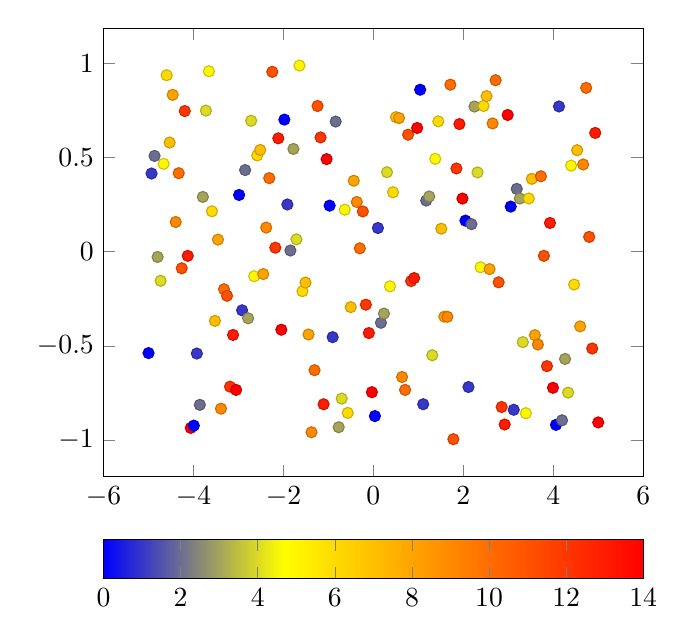
\begin{tikzpicture}
            \begin{axis}[colorbar horizontal]
              \addplot[only marks,scatter,
                scatter src={mod(\coordindex,15)},samples=150]
                {rand};
            \end{axis}
        \end{tikzpicture}}
      \end{center}
    \end{figure}
  \end{minipage}

  \vspace*{.1in}
  \tikzstyle{proc} = [draw, thick, fill=solarizedViolet, text centered, rounded corners,
    text=solarizedRebase02, draw=solarizedViolet]

\tikzstyle{prochighlight} = [draw, thick, fill=solarizedOrange, text centered, rounded corners,
    text=solarizedRebase02, draw=solarizedOrange]

\tikzstyle{procold} = [draw, thick, fill=solarizedViolet!75, text centered, rounded corners,
    text=solarizedRebase02, draw=solarizedViolet!75]

\tikzstyle{procchanged} = [draw, thick, fill=solarizedViolet!75, text centered, rounded corners,
    text=solarizedRebase02, draw=solarizedViolet!75]

\tikzstyle{prochighlightold} = [draw, thick, fill=solarizedOrange!75, text centered, rounded corners,
    text=solarizedRebase02, draw=solarizedOrange!75]

\tikzstyle{prochighlightchanged} = [draw, thick, fill=solarizedYellow!75, text centered, rounded corners,
    text=solarizedRebase02, draw=solarizedYellow!75]

\tikzstyle{proctest} = [draw, thick, fill=solarizedOrange, text centered, rounded corners,
text=solarizedBase02, draw=solarizedOrange]

\tikzstyle{procnew} = [draw, thick, fill=solarizedGreen, text centered, rounded corners,
    text=solarizedRebase02, draw=solarizedGreen]

\tikzstyle{procyellow} = [draw, thick, fill=solarizedYellow, text centered, rounded corners,
    text=solarizedRebase02, draw=solarizedYellow]

\tikzstyle{procred} = [draw, thick, fill=solarizedRed, text centered, rounded corners,
    text=solarizedRebase02, draw=solarizedRed]

\tikzstyle{io} = [ellipse, draw, thick, fill=solarizedBlue, draw=solarizedBlue, text=solarizedRebase02]

\tikzstyle{iopass} = [ellipse, draw, thick, fill=solarizedGreen, draw=solarizedGreen, text=solarizedRebase02]
\tikzstyle{iofail} = [ellipse, draw, thick, fill=solarizedRed, draw=solarizedRed, text=solarizedRebase02]
\tikzstyle{iohighlight} = [ellipse, draw, thick, fill=solarizedYellow, draw=solarizedYellow,
    text=solarizedRebase02]

\tikzstyle{iofailother} = [ellipse, draw, thick, fill=solarizedYellow, draw=solarizedYellow,
    text=solarizedRebase02]
\tikzstyle{wrongoutput} = [ellipse, draw, thick, fill=solarizedCyan, draw=solarizedCyan, text=solarizedRebase02]

\tikzstyle{special} = [draw, thick, fill=solarizedGreen, text centered, draw=solarizedGreen,
    text=solarizedBase02]
\tikzstyle{specialOrange} = [draw, thick, fill=solarizedOrange, text centered, draw=solarizedOrange,
    text=solarizedBase02]
\tikzstyle{specialGreen} = [draw, thick, fill=solarizedGreen, text centered, draw=solarizedGreen,
    text=solarizedBase02]
\tikzstyle{specialYellow} = [draw, thick, fill=solarizedYellow, text centered, draw=solarizedYellow,
    text=solarizedBase02]

\tikzstyle{pass} = [draw, thick, fill=solarizedGreen, text centered, draw=solarizedGreen, text=solarizedRebase02]
\tikzstyle{fail} = [draw, thick, fill=solarizedRed, text centered, draw=solarizedRed, text=solarizedRebase02]

\tikzstyle{feature} = [draw, thick, fill=solarizedOrange, text centered, text=solarizedRebase02, draw=solarizedOrange]

\tikzstyle{plain} = [draw, thick, fill=kapfhammerDarkGrey, text centered, text=solarizedRebase02, draw=kapfhammerDarkGrey]
\tikzstyle{featurecurve} = [draw, thick, fill=solarizedGreen, text centered, rounded corners]

  \begin{figure}
    \begin{centering}
      \begin{tikzpicture}
        \path[->]<2-> node[special,]
          (Requirements) at (0,1.0)
          {Easy to implement --- and yet not always very effective!};
      \end{tikzpicture}
    \end{centering}
  \end{figure}

\end{frame}

\begin{frame}[t]
  \frametitle{Search-Based Testing}
  \framesubtitle{\mbox{}}

  % \vspace*{.25in}
  \hspace{.50in}
  \begin{minipage}{3.0in}
    \begin{figure}
      \resizebox{3.0in}{!}{
        \begin{tikzpicture}
          \begin{axis}[
              domain=0:1,
              xmax=1,
              ymax=1,
            ]
            \addplot3[surf] {x*y};
            \addplot3[solarizedRebase0,/pgfplots/quiver,
                quiver/u=y,
                quiver/v=x,
                quiver/w=0,
                quiver/scale arrows=0.1,
              -stealth,samples=10] {1};
          \end{axis}
      \end{tikzpicture}}
    \end{figure}
  \end{minipage}

  \vspace*{.1in}
  \tikzstyle{proc} = [draw, thick, fill=solarizedViolet, text centered, rounded corners,
    text=solarizedRebase02, draw=solarizedViolet]

\tikzstyle{prochighlight} = [draw, thick, fill=solarizedOrange, text centered, rounded corners,
    text=solarizedRebase02, draw=solarizedOrange]

\tikzstyle{procold} = [draw, thick, fill=solarizedViolet!75, text centered, rounded corners,
    text=solarizedRebase02, draw=solarizedViolet!75]

\tikzstyle{procchanged} = [draw, thick, fill=solarizedViolet!75, text centered, rounded corners,
    text=solarizedRebase02, draw=solarizedViolet!75]

\tikzstyle{prochighlightold} = [draw, thick, fill=solarizedOrange!75, text centered, rounded corners,
    text=solarizedRebase02, draw=solarizedOrange!75]

\tikzstyle{prochighlightchanged} = [draw, thick, fill=solarizedYellow!75, text centered, rounded corners,
    text=solarizedRebase02, draw=solarizedYellow!75]

\tikzstyle{proctest} = [draw, thick, fill=solarizedOrange, text centered, rounded corners,
text=solarizedBase02, draw=solarizedOrange]

\tikzstyle{procnew} = [draw, thick, fill=solarizedGreen, text centered, rounded corners,
    text=solarizedRebase02, draw=solarizedGreen]

\tikzstyle{procyellow} = [draw, thick, fill=solarizedYellow, text centered, rounded corners,
    text=solarizedRebase02, draw=solarizedYellow]

\tikzstyle{procred} = [draw, thick, fill=solarizedRed, text centered, rounded corners,
    text=solarizedRebase02, draw=solarizedRed]

\tikzstyle{io} = [ellipse, draw, thick, fill=solarizedBlue, draw=solarizedBlue, text=solarizedRebase02]

\tikzstyle{iopass} = [ellipse, draw, thick, fill=solarizedGreen, draw=solarizedGreen, text=solarizedRebase02]
\tikzstyle{iofail} = [ellipse, draw, thick, fill=solarizedRed, draw=solarizedRed, text=solarizedRebase02]
\tikzstyle{iohighlight} = [ellipse, draw, thick, fill=solarizedYellow, draw=solarizedYellow,
    text=solarizedRebase02]

\tikzstyle{iofailother} = [ellipse, draw, thick, fill=solarizedYellow, draw=solarizedYellow,
    text=solarizedRebase02]
\tikzstyle{wrongoutput} = [ellipse, draw, thick, fill=solarizedCyan, draw=solarizedCyan, text=solarizedRebase02]

\tikzstyle{special} = [draw, thick, fill=solarizedGreen, text centered, draw=solarizedGreen,
    text=solarizedBase02]
\tikzstyle{specialOrange} = [draw, thick, fill=solarizedOrange, text centered, draw=solarizedOrange,
    text=solarizedBase02]
\tikzstyle{specialGreen} = [draw, thick, fill=solarizedGreen, text centered, draw=solarizedGreen,
    text=solarizedBase02]
\tikzstyle{specialYellow} = [draw, thick, fill=solarizedYellow, text centered, draw=solarizedYellow,
    text=solarizedBase02]

\tikzstyle{pass} = [draw, thick, fill=solarizedGreen, text centered, draw=solarizedGreen, text=solarizedRebase02]
\tikzstyle{fail} = [draw, thick, fill=solarizedRed, text centered, draw=solarizedRed, text=solarizedRebase02]

\tikzstyle{feature} = [draw, thick, fill=solarizedOrange, text centered, text=solarizedRebase02, draw=solarizedOrange]

\tikzstyle{plain} = [draw, thick, fill=kapfhammerDarkGrey, text centered, text=solarizedRebase02, draw=kapfhammerDarkGrey]
\tikzstyle{featurecurve} = [draw, thick, fill=solarizedGreen, text centered, rounded corners]

  \begin{figure}
    \begin{centering}
      \begin{tikzpicture}
        \path[->]<2-> node[special,]
          (Requirements) at (0,.75)
          {Often much more effective than random testing};
      \end{tikzpicture}
    \end{centering}
  \end{figure}

\end{frame}

\begin{frame}
  \frametitle{Performance of SBST}
  \framesubtitle{\mbox{}}
  \tikzstyle{proc} = [draw, thick, fill=solarizedViolet, text centered, rounded corners,
    text=solarizedRebase02, draw=solarizedViolet]

\tikzstyle{prochighlight} = [draw, thick, fill=solarizedOrange, text centered, rounded corners,
    text=solarizedRebase02, draw=solarizedOrange]

\tikzstyle{procold} = [draw, thick, fill=solarizedViolet!75, text centered, rounded corners,
    text=solarizedRebase02, draw=solarizedViolet!75]

\tikzstyle{procchanged} = [draw, thick, fill=solarizedViolet!75, text centered, rounded corners,
    text=solarizedRebase02, draw=solarizedViolet!75]

\tikzstyle{prochighlightold} = [draw, thick, fill=solarizedOrange!75, text centered, rounded corners,
    text=solarizedRebase02, draw=solarizedOrange!75]

\tikzstyle{prochighlightchanged} = [draw, thick, fill=solarizedYellow!75, text centered, rounded corners,
    text=solarizedRebase02, draw=solarizedYellow!75]

\tikzstyle{proctest} = [draw, thick, fill=solarizedOrange, text centered, rounded corners,
text=solarizedBase02, draw=solarizedOrange]

\tikzstyle{procnew} = [draw, thick, fill=solarizedGreen, text centered, rounded corners,
    text=solarizedRebase02, draw=solarizedGreen]

\tikzstyle{procyellow} = [draw, thick, fill=solarizedYellow, text centered, rounded corners,
    text=solarizedRebase02, draw=solarizedYellow]

\tikzstyle{procred} = [draw, thick, fill=solarizedRed, text centered, rounded corners,
    text=solarizedRebase02, draw=solarizedRed]

\tikzstyle{io} = [ellipse, draw, thick, fill=solarizedBlue, draw=solarizedBlue, text=solarizedRebase02]

\tikzstyle{iopass} = [ellipse, draw, thick, fill=solarizedGreen, draw=solarizedGreen, text=solarizedRebase02]
\tikzstyle{iofail} = [ellipse, draw, thick, fill=solarizedRed, draw=solarizedRed, text=solarizedRebase02]
\tikzstyle{iohighlight} = [ellipse, draw, thick, fill=solarizedYellow, draw=solarizedYellow,
    text=solarizedRebase02]

\tikzstyle{iofailother} = [ellipse, draw, thick, fill=solarizedYellow, draw=solarizedYellow,
    text=solarizedRebase02]
\tikzstyle{wrongoutput} = [ellipse, draw, thick, fill=solarizedCyan, draw=solarizedCyan, text=solarizedRebase02]

\tikzstyle{special} = [draw, thick, fill=solarizedGreen, text centered, draw=solarizedGreen,
    text=solarizedBase02]
\tikzstyle{specialOrange} = [draw, thick, fill=solarizedOrange, text centered, draw=solarizedOrange,
    text=solarizedBase02]
\tikzstyle{specialGreen} = [draw, thick, fill=solarizedGreen, text centered, draw=solarizedGreen,
    text=solarizedBase02]
\tikzstyle{specialYellow} = [draw, thick, fill=solarizedYellow, text centered, draw=solarizedYellow,
    text=solarizedBase02]

\tikzstyle{pass} = [draw, thick, fill=solarizedGreen, text centered, draw=solarizedGreen, text=solarizedRebase02]
\tikzstyle{fail} = [draw, thick, fill=solarizedRed, text centered, draw=solarizedRed, text=solarizedRebase02]

\tikzstyle{feature} = [draw, thick, fill=solarizedOrange, text centered, text=solarizedRebase02, draw=solarizedOrange]

\tikzstyle{plain} = [draw, thick, fill=kapfhammerDarkGrey, text centered, text=solarizedRebase02, draw=kapfhammerDarkGrey]
\tikzstyle{featurecurve} = [draw, thick, fill=solarizedGreen, text centered, rounded corners]

  %!TEX root=kinneer_seke.tex
% mainfile: kinneer_seke.tex

%%%%%%%%%%%%%%%%%%%%%%%%%%%%%%%%%%%%%%%%%%%%%%%%%%%%%%%%%%%%%%%
% Arithmetic of the clock
% Author: Juan Luis Varona
% http://www.unirioja.es/cu/jvarona/
%%%<
%%%>
% :Title: Arithmetic of the clock
% :Author: Juan Luis Varona
%
% This example shows the products i times j for
% i and j from 0 to 11 by using arithmetic modulo 12,
% i.e., the so called arithmetic of the clock.
%

% The results of the products are represented both by
% the color of the clock and by the hand.
% Colors:

% \definecolor{clock0}{cmyk}{1,0,0,0} % cyan
\definecolor{clock0}{HTML}{CB4B16}

\definecolor{clock1}{cmyk}{0.75,0.25,0,0}
\definecolor{clock2}{cmyk}{0.5,0.5,0,0}

% \definecolor{clock3}{cmyk}{0.25,0.75,0,0}
\definecolor{clock3}{HTML}{DC322F}

\definecolor{clock4}{cmyk}{0,1,0,0} % magenta
\definecolor{clock5}{cmyk}{0,0.75,0.25,0}
\definecolor{clock6}{cmyk}{0,0,5,0.5,0}
\definecolor{clock7}{cmyk}{0,0.25,0.75,0}
\definecolor{clock8}{cmyk}{0,0,1,0} % yellow

% \definecolor{clock9}{cmyk}{0.25,0,0.75,0}
\definecolor{clock9}{HTML}{6C71C4}

\definecolor{clock10}{cmyk}{0.5,0,0.5,0}

% \definecolor{clock11}{cmyk}{0.75,0,0.25,0}
\definecolor{clock11}{HTML}{268BD2}

% x pos, y pos, color, hand position
\newcommand{\clock}[4]{%
  \begin{scope}[xshift=2.25*#1cm,yshift=2.25*#2cm]
  % \filldraw [fill=#3, line width=1.6pt] (0,0) circle (1cm); % simple fill (unused)
  % \draw[fill] (0,0) circle (1mm); % border (unused)
  \shadedraw [inner color=#3!30!white, outer color=#3!90!black,
    line width=1.6pt] (0,0) circle (1cm); % disk with shadow and border
  \foreach \angle in {0, 30, ..., 330}
    \draw[line width=1pt] (\angle:0.82cm) -- (\angle:1cm);
  \foreach \angle in {0,90,180,270}
    \draw[line width=1.3pt] (\angle:0.75cm) -- (\angle:1cm);
  \draw[line width=1.6pt] (0,0) -- (90-30*#4:0.6cm); % the hand
  \end{scope}
}

\setbeamercovered{invisible}

\hspace*{.125in}
\begin{overprint}[5.0in]
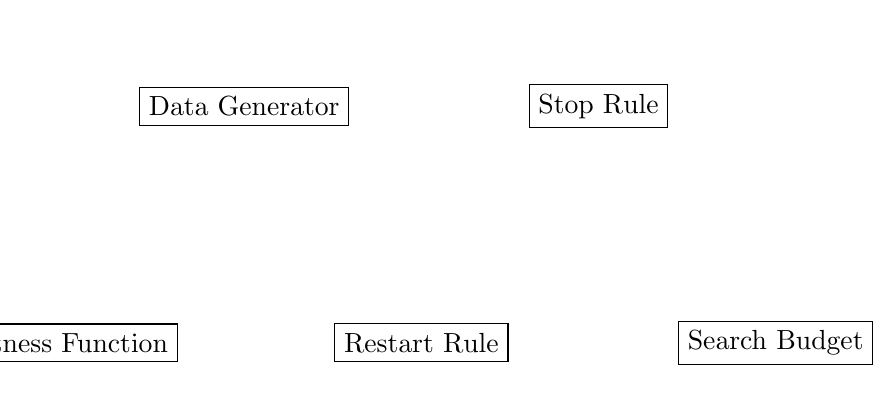
\begin{tikzpicture}[scale=1]

  \path[use as bounding box] (-0.5,2.5) rectangle (10,-2);

  \uncover<2->{
    \clock{0}{0}{clock0}{8};
    \node[draw] at (0cm,-1.5cm) {Fitness Function};
  }
  \uncover<3->{
    \clock{1}{0}{clock3}{1};
    \node[draw] at (2.25cm,+1.5cm) {Data Generator};
  }
  \uncover<4->{
    \clock{2}{0}{clock6}{6};
    \node[draw] at (4.50cm,-1.5cm) {Restart Rule};
  }
  \uncover<5->{
    \clock{3}{0}{clock9}{11};
    \node[draw] at (6.75cm,+1.5cm) {Stop Rule};
  }
  \uncover<6->{
    \clock{4}{0}{clock11}{10};
    \node[draw] at (9cm,-1.5cm) {Search Budget};
  }

\end{tikzpicture}

\hspace*{.33in}
\begin{tikzpicture}
  \path[use as bounding box] (-4.5,1) rectangle (10,-2);
  \path[->]<7-> node[special, text width=40ex]
    (Requirements) at (0,-.6)
    {{\Large How do parameter values \\ influence the efficiency of SBST?}};

\end{tikzpicture}

\end{overprint}

\end{frame}

\setbeamercovered{invisible}
\begin{frame}%[label=current]
  \frametitle{Performance of SBST}
  \framesubtitle{\mbox{}}

  \vspace*{.3in}
  \begin{center}
    \fontsize{90}{72}\selectfont
    O(\uncover<2->{\textcolor{solarizedViolet}{?}})
  \end{center}

  \tikzstyle{proc} = [draw, thick, fill=solarizedViolet, text centered, rounded corners,
    text=solarizedRebase02, draw=solarizedViolet]

\tikzstyle{prochighlight} = [draw, thick, fill=solarizedOrange, text centered, rounded corners,
    text=solarizedRebase02, draw=solarizedOrange]

\tikzstyle{procold} = [draw, thick, fill=solarizedViolet!75, text centered, rounded corners,
    text=solarizedRebase02, draw=solarizedViolet!75]

\tikzstyle{procchanged} = [draw, thick, fill=solarizedViolet!75, text centered, rounded corners,
    text=solarizedRebase02, draw=solarizedViolet!75]

\tikzstyle{prochighlightold} = [draw, thick, fill=solarizedOrange!75, text centered, rounded corners,
    text=solarizedRebase02, draw=solarizedOrange!75]

\tikzstyle{prochighlightchanged} = [draw, thick, fill=solarizedYellow!75, text centered, rounded corners,
    text=solarizedRebase02, draw=solarizedYellow!75]

\tikzstyle{proctest} = [draw, thick, fill=solarizedOrange, text centered, rounded corners,
text=solarizedBase02, draw=solarizedOrange]

\tikzstyle{procnew} = [draw, thick, fill=solarizedGreen, text centered, rounded corners,
    text=solarizedRebase02, draw=solarizedGreen]

\tikzstyle{procyellow} = [draw, thick, fill=solarizedYellow, text centered, rounded corners,
    text=solarizedRebase02, draw=solarizedYellow]

\tikzstyle{procred} = [draw, thick, fill=solarizedRed, text centered, rounded corners,
    text=solarizedRebase02, draw=solarizedRed]

\tikzstyle{io} = [ellipse, draw, thick, fill=solarizedBlue, draw=solarizedBlue, text=solarizedRebase02]

\tikzstyle{iopass} = [ellipse, draw, thick, fill=solarizedGreen, draw=solarizedGreen, text=solarizedRebase02]
\tikzstyle{iofail} = [ellipse, draw, thick, fill=solarizedRed, draw=solarizedRed, text=solarizedRebase02]
\tikzstyle{iohighlight} = [ellipse, draw, thick, fill=solarizedYellow, draw=solarizedYellow,
    text=solarizedRebase02]

\tikzstyle{iofailother} = [ellipse, draw, thick, fill=solarizedYellow, draw=solarizedYellow,
    text=solarizedRebase02]
\tikzstyle{wrongoutput} = [ellipse, draw, thick, fill=solarizedCyan, draw=solarizedCyan, text=solarizedRebase02]

\tikzstyle{special} = [draw, thick, fill=solarizedGreen, text centered, draw=solarizedGreen,
    text=solarizedBase02]
\tikzstyle{specialOrange} = [draw, thick, fill=solarizedOrange, text centered, draw=solarizedOrange,
    text=solarizedBase02]
\tikzstyle{specialGreen} = [draw, thick, fill=solarizedGreen, text centered, draw=solarizedGreen,
    text=solarizedBase02]
\tikzstyle{specialYellow} = [draw, thick, fill=solarizedYellow, text centered, draw=solarizedYellow,
    text=solarizedBase02]

\tikzstyle{pass} = [draw, thick, fill=solarizedGreen, text centered, draw=solarizedGreen, text=solarizedRebase02]
\tikzstyle{fail} = [draw, thick, fill=solarizedRed, text centered, draw=solarizedRed, text=solarizedRebase02]

\tikzstyle{feature} = [draw, thick, fill=solarizedOrange, text centered, text=solarizedRebase02, draw=solarizedOrange]

\tikzstyle{plain} = [draw, thick, fill=kapfhammerDarkGrey, text centered, text=solarizedRebase02, draw=kapfhammerDarkGrey]
\tikzstyle{featurecurve} = [draw, thick, fill=solarizedGreen, text centered, rounded corners]

  \begin{tikzpicture}
    \path[use as bounding box] (-5.5,1) rectangle (10,-2);

          \path[->]<3> node[plain, text width=20ex]
          (Theoretical) at (-2.75,-.25) {\Huge \xmarkhide {Analytical}};

          \path[->]<4-> node[plain, text width=20ex]
          (Theoretical) at (-2.75,-.25) {\Huge \xmark {Analytical}};

          \path[->]<5> node[plain,right of=Theoretical,
          yshift=-0.0in, xshift=1.75in, minimum width=20ex]
                      (Empirical) {\Huge \cmarkhide {Empirical}};

          \path[->]<6-> node[plain,right of=Theoretical,
          yshift=-0.0in, xshift=1.75in, minimum width=20ex]
                      (Empirical) {\Huge \cmark {Empirical}};

  \end{tikzpicture}
\end{frame}


\section{Background}
\begin{frame}
  \frametitle{Doubling Experiment}

  \tikzstyle{proc} = [draw, thick, fill=solarizedViolet, text centered, rounded corners,
    text=solarizedRebase02, draw=solarizedViolet]

\tikzstyle{prochighlight} = [draw, thick, fill=solarizedOrange, text centered, rounded corners,
    text=solarizedRebase02, draw=solarizedOrange]

\tikzstyle{procold} = [draw, thick, fill=solarizedViolet!75, text centered, rounded corners,
    text=solarizedRebase02, draw=solarizedViolet!75]

\tikzstyle{procchanged} = [draw, thick, fill=solarizedViolet!75, text centered, rounded corners,
    text=solarizedRebase02, draw=solarizedViolet!75]

\tikzstyle{prochighlightold} = [draw, thick, fill=solarizedOrange!75, text centered, rounded corners,
    text=solarizedRebase02, draw=solarizedOrange!75]

\tikzstyle{prochighlightchanged} = [draw, thick, fill=solarizedYellow!75, text centered, rounded corners,
    text=solarizedRebase02, draw=solarizedYellow!75]

\tikzstyle{proctest} = [draw, thick, fill=solarizedOrange, text centered, rounded corners,
text=solarizedBase02, draw=solarizedOrange]

\tikzstyle{procnew} = [draw, thick, fill=solarizedGreen, text centered, rounded corners,
    text=solarizedRebase02, draw=solarizedGreen]

\tikzstyle{procyellow} = [draw, thick, fill=solarizedYellow, text centered, rounded corners,
    text=solarizedRebase02, draw=solarizedYellow]

\tikzstyle{procred} = [draw, thick, fill=solarizedRed, text centered, rounded corners,
    text=solarizedRebase02, draw=solarizedRed]

\tikzstyle{io} = [ellipse, draw, thick, fill=solarizedBlue, draw=solarizedBlue, text=solarizedRebase02]

\tikzstyle{iopass} = [ellipse, draw, thick, fill=solarizedGreen, draw=solarizedGreen, text=solarizedRebase02]
\tikzstyle{iofail} = [ellipse, draw, thick, fill=solarizedRed, draw=solarizedRed, text=solarizedRebase02]
\tikzstyle{iohighlight} = [ellipse, draw, thick, fill=solarizedYellow, draw=solarizedYellow,
    text=solarizedRebase02]

\tikzstyle{iofailother} = [ellipse, draw, thick, fill=solarizedYellow, draw=solarizedYellow,
    text=solarizedRebase02]
\tikzstyle{wrongoutput} = [ellipse, draw, thick, fill=solarizedCyan, draw=solarizedCyan, text=solarizedRebase02]

\tikzstyle{special} = [draw, thick, fill=solarizedGreen, text centered, draw=solarizedGreen,
    text=solarizedBase02]
\tikzstyle{specialOrange} = [draw, thick, fill=solarizedOrange, text centered, draw=solarizedOrange,
    text=solarizedBase02]
\tikzstyle{specialGreen} = [draw, thick, fill=solarizedGreen, text centered, draw=solarizedGreen,
    text=solarizedBase02]
\tikzstyle{specialYellow} = [draw, thick, fill=solarizedYellow, text centered, draw=solarizedYellow,
    text=solarizedBase02]

\tikzstyle{pass} = [draw, thick, fill=solarizedGreen, text centered, draw=solarizedGreen, text=solarizedRebase02]
\tikzstyle{fail} = [draw, thick, fill=solarizedRed, text centered, draw=solarizedRed, text=solarizedRebase02]

\tikzstyle{feature} = [draw, thick, fill=solarizedOrange, text centered, text=solarizedRebase02, draw=solarizedOrange]

\tikzstyle{plain} = [draw, thick, fill=kapfhammerDarkGrey, text centered, text=solarizedRebase02, draw=kapfhammerDarkGrey]
\tikzstyle{featurecurve} = [draw, thick, fill=solarizedGreen, text centered, rounded corners]

  \hspace{-.25in}

  \begin{center}

    \begin{tikzpicture}[thick,scale=1, every node/.style={scale=1}]

      \path[use as bounding box] (-3.0,2.5) rectangle (10,-2);

      \path[->]<1,4-> node[proc, minimum width=7ex]
      (input1) at (0,1.5) {Input};

      \path[->]<2-3> node[proctest, minimum width=7ex]
      (input1) at (0,1.5) {Input};

      \path[->]<3-> node[io, below of=input1, yshift=-0.3in,
      xshift=0.0in,minimum width=11ex] 
      (runtime1) {Runtime = 1};


      \path[->]<4,7-> node[proc, right of=input1, yshift=0.0in,
      xshift=1.25in,minimum width=7ex,minimum height=4*\heightof{Input}] 
      (input2) {Input};

      
      \path[->]<5-6> node[proctest, right of=input1, yshift=0.0in,
      xshift=1.25in,minimum width=7ex,minimum height=4*\heightof{Input}] 
      (input2) {Input};


      \path[->]<6-> node[io, below of=input2, yshift=-0.3in,
      xshift=0.0in,minimum width=11ex] 
      (runtime2) {Runtime = 2};

      \path[->]<8-> node[io, below of=input1, yshift=-0.6in,
      xshift=0.75in,minimum width=11ex] 
      (ratio) {Ratio = 2};

      \path[->]<9-> node[special, below of=ratio, yshift=-0.3in,
      xshift=0.0in,minimum width=11ex] 
      (takeaway) {LINEAR};





    \end{tikzpicture}

  \end{center}

\end{frame}


\section{Technique}
\begin{frame}
    \frametitle{Method of Approach}
    \centering
    \tikzstyle{proc} = [draw, thick, fill=solarizedViolet, text centered, rounded corners,
    text=solarizedRebase02, draw=solarizedViolet]

\tikzstyle{prochighlight} = [draw, thick, fill=solarizedOrange, text centered, rounded corners,
    text=solarizedRebase02, draw=solarizedOrange]

\tikzstyle{procold} = [draw, thick, fill=solarizedViolet!75, text centered, rounded corners,
    text=solarizedRebase02, draw=solarizedViolet!75]

\tikzstyle{procchanged} = [draw, thick, fill=solarizedViolet!75, text centered, rounded corners,
    text=solarizedRebase02, draw=solarizedViolet!75]

\tikzstyle{prochighlightold} = [draw, thick, fill=solarizedOrange!75, text centered, rounded corners,
    text=solarizedRebase02, draw=solarizedOrange!75]

\tikzstyle{prochighlightchanged} = [draw, thick, fill=solarizedYellow!75, text centered, rounded corners,
    text=solarizedRebase02, draw=solarizedYellow!75]

\tikzstyle{proctest} = [draw, thick, fill=solarizedOrange, text centered, rounded corners,
text=solarizedBase02, draw=solarizedOrange]

\tikzstyle{procnew} = [draw, thick, fill=solarizedGreen, text centered, rounded corners,
    text=solarizedRebase02, draw=solarizedGreen]

\tikzstyle{procyellow} = [draw, thick, fill=solarizedYellow, text centered, rounded corners,
    text=solarizedRebase02, draw=solarizedYellow]

\tikzstyle{procred} = [draw, thick, fill=solarizedRed, text centered, rounded corners,
    text=solarizedRebase02, draw=solarizedRed]

\tikzstyle{io} = [ellipse, draw, thick, fill=solarizedBlue, draw=solarizedBlue, text=solarizedRebase02]

\tikzstyle{iopass} = [ellipse, draw, thick, fill=solarizedGreen, draw=solarizedGreen, text=solarizedRebase02]
\tikzstyle{iofail} = [ellipse, draw, thick, fill=solarizedRed, draw=solarizedRed, text=solarizedRebase02]
\tikzstyle{iohighlight} = [ellipse, draw, thick, fill=solarizedYellow, draw=solarizedYellow,
    text=solarizedRebase02]

\tikzstyle{iofailother} = [ellipse, draw, thick, fill=solarizedYellow, draw=solarizedYellow,
    text=solarizedRebase02]
\tikzstyle{wrongoutput} = [ellipse, draw, thick, fill=solarizedCyan, draw=solarizedCyan, text=solarizedRebase02]

\tikzstyle{special} = [draw, thick, fill=solarizedGreen, text centered, draw=solarizedGreen,
    text=solarizedBase02]
\tikzstyle{specialOrange} = [draw, thick, fill=solarizedOrange, text centered, draw=solarizedOrange,
    text=solarizedBase02]
\tikzstyle{specialGreen} = [draw, thick, fill=solarizedGreen, text centered, draw=solarizedGreen,
    text=solarizedBase02]
\tikzstyle{specialYellow} = [draw, thick, fill=solarizedYellow, text centered, draw=solarizedYellow,
    text=solarizedBase02]

\tikzstyle{pass} = [draw, thick, fill=solarizedGreen, text centered, draw=solarizedGreen, text=solarizedRebase02]
\tikzstyle{fail} = [draw, thick, fill=solarizedRed, text centered, draw=solarizedRed, text=solarizedRebase02]

\tikzstyle{feature} = [draw, thick, fill=solarizedOrange, text centered, text=solarizedRebase02, draw=solarizedOrange]

\tikzstyle{plain} = [draw, thick, fill=kapfhammerDarkGrey, text centered, text=solarizedRebase02, draw=kapfhammerDarkGrey]
\tikzstyle{featurecurve} = [draw, thick, fill=solarizedGreen, text centered, rounded corners]

    \newcommand{\mx}[1]{\mathbf{\bm{#1}}} % Matrix command
\newcommand{\vc}[1]{\mathbf{\bm{#1}}} % Vector command

% Define the layers to draw the diagram
\pgfdeclarelayer{background}
\pgfdeclarelayer{foreground}
\pgfsetlayers{background,main,foreground}

% Define distances for bordering
\def\blockdist{3.5}
\def\vertdist{2}

\hspace{-.25in}

\begin{minipage}{5in}

  \begin{center}

    \vspace*{-.3in}
    \begin{minipage}{4.5in}

      \begin{figure}

        \begin{center}

\begin{tikzpicture}[thick,scale=1, every node/.style={scale=1}]

  \path[use as bounding box] (-3.0,2.5) rectangle (10,-2);

    \path[->]<1-> node[proc, text width=15ex]
    (sa) at (1.5,.75) {\centering \textit{SchemaAnalyst} \\ Execution};

    \path[->]<2-> node[io, left of=sa, yshift=0.70in, xshift=-1.25in,text width=7ex]
    (cc) {\centering Coverage \\ Criterion} (cc) edge node {} (sa);

    \path[->]<3-> node[io, left of=sa, yshift=0.0in, xshift=-1.25in,text width=7ex]
    (dg) {\centering Data \\ Generator} (dg) edge node {} (sa);

    \path[->]<4-6> node[io, left of=sa, yshift=-0.70in, xshift=-1.25in,text width=7ex]
    (ds) {\centering Database \\ Schema} (ds) edge node {} (sa);

    \path[->]<5> node[io, right of=sa, yshift=0.0in, xshift=1.25in,text width=7ex]
    (ts) {\centering Test \\ Suite \\} (sa) edge node {} (ts);

    \path[->]<6-> node[io, right of=sa, yshift=0.0in, xshift=1.25in,text width=7ex]
    (ts) {\centering Runtime} (sa) edge node {} (ts);

    \path[->]<7-> node[proc, below of=sa, yshift=-0.3in, xshift=0.0in,text width=15ex]
    (sd) {\centering Schema Doubler} (sd) edge node {Provides Schema} (sa);

    \path[->]<7-> node[io, left of=sa, yshift=-0.70in, xshift=-1.25in,text width=7ex]
    (ds) {\centering Database \\ Schema} (ds) edge node {} (sd);

    \path[->]<8-> node[io, left of=sa, yshift=-1.40in, xshift=-1.25in,text width=7ex]
    (dc) {\centering Doubler \\ Choice} (dc) edge node {} (sd);

    \path[->]<9-> node[proc, right of=sd, yshift=0.0in, xshift=1.25in,text width=15ex]
    (ca) {\centering Convergence \\ Algorithm} (ca) edge node [below=.20in]{Continue?} (sd);

    \path[->]<9-> (ts) edge node {} (ca);


\end{tikzpicture}

\end{center}

\end{figure}

\end{minipage}

\end{center}

\end{minipage}

\end{frame}

\begin{frame}
    \frametitle{Doubling Database Schemas}
    \centering
    \tikzstyle{proc} = [draw, thick, fill=solarizedViolet, text centered, rounded corners,
    text=solarizedRebase02, draw=solarizedViolet]

\tikzstyle{prochighlight} = [draw, thick, fill=solarizedOrange, text centered, rounded corners,
    text=solarizedRebase02, draw=solarizedOrange]

\tikzstyle{procold} = [draw, thick, fill=solarizedViolet!75, text centered, rounded corners,
    text=solarizedRebase02, draw=solarizedViolet!75]

\tikzstyle{procchanged} = [draw, thick, fill=solarizedViolet!75, text centered, rounded corners,
    text=solarizedRebase02, draw=solarizedViolet!75]

\tikzstyle{prochighlightold} = [draw, thick, fill=solarizedOrange!75, text centered, rounded corners,
    text=solarizedRebase02, draw=solarizedOrange!75]

\tikzstyle{prochighlightchanged} = [draw, thick, fill=solarizedYellow!75, text centered, rounded corners,
    text=solarizedRebase02, draw=solarizedYellow!75]

\tikzstyle{proctest} = [draw, thick, fill=solarizedOrange, text centered, rounded corners,
text=solarizedBase02, draw=solarizedOrange]

\tikzstyle{procnew} = [draw, thick, fill=solarizedGreen, text centered, rounded corners,
    text=solarizedRebase02, draw=solarizedGreen]

\tikzstyle{procyellow} = [draw, thick, fill=solarizedYellow, text centered, rounded corners,
    text=solarizedRebase02, draw=solarizedYellow]

\tikzstyle{procred} = [draw, thick, fill=solarizedRed, text centered, rounded corners,
    text=solarizedRebase02, draw=solarizedRed]

\tikzstyle{io} = [ellipse, draw, thick, fill=solarizedBlue, draw=solarizedBlue, text=solarizedRebase02]

\tikzstyle{iopass} = [ellipse, draw, thick, fill=solarizedGreen, draw=solarizedGreen, text=solarizedRebase02]
\tikzstyle{iofail} = [ellipse, draw, thick, fill=solarizedRed, draw=solarizedRed, text=solarizedRebase02]
\tikzstyle{iohighlight} = [ellipse, draw, thick, fill=solarizedYellow, draw=solarizedYellow,
    text=solarizedRebase02]

\tikzstyle{iofailother} = [ellipse, draw, thick, fill=solarizedYellow, draw=solarizedYellow,
    text=solarizedRebase02]
\tikzstyle{wrongoutput} = [ellipse, draw, thick, fill=solarizedCyan, draw=solarizedCyan, text=solarizedRebase02]

\tikzstyle{special} = [draw, thick, fill=solarizedGreen, text centered, draw=solarizedGreen,
    text=solarizedBase02]
\tikzstyle{specialOrange} = [draw, thick, fill=solarizedOrange, text centered, draw=solarizedOrange,
    text=solarizedBase02]
\tikzstyle{specialGreen} = [draw, thick, fill=solarizedGreen, text centered, draw=solarizedGreen,
    text=solarizedBase02]
\tikzstyle{specialYellow} = [draw, thick, fill=solarizedYellow, text centered, draw=solarizedYellow,
    text=solarizedBase02]

\tikzstyle{pass} = [draw, thick, fill=solarizedGreen, text centered, draw=solarizedGreen, text=solarizedRebase02]
\tikzstyle{fail} = [draw, thick, fill=solarizedRed, text centered, draw=solarizedRed, text=solarizedRebase02]

\tikzstyle{feature} = [draw, thick, fill=solarizedOrange, text centered, text=solarizedRebase02, draw=solarizedOrange]

\tikzstyle{plain} = [draw, thick, fill=kapfhammerDarkGrey, text centered, text=solarizedRebase02, draw=kapfhammerDarkGrey]
\tikzstyle{featurecurve} = [draw, thick, fill=solarizedGreen, text centered, rounded corners]

    \pgfdeclarelayer{background}
\pgfdeclarelayer{foreground}
\pgfsetlayers{background,main,foreground}

\begin{minipage}{.5in}

\begin{center}

\begin{minipage}{.45in}

\begin{figure}

\begin{center}

\begin{tikzpicture}[thick,scale=1, every node/.style={scale=1}]

\path[use as bounding box] (-5.0,2.5) rectangle (10,-2);

\node<1-> (table) [proc] {
    \begin{tabular}{l}
    \textbf{Table}\\ \hline
        \parbox{4cm}{
            \begin{itemize}
                \color{solarizedBase02}
                \item Column 1
                \item Column 2
                \item \dots
                \item Column n
            \end{itemize}
        }
    \end{tabular}
};

\path<2-> (table.west)+(-2,0) node (nn1) [proctest] {NOT NULL};
\path<2-> [draw, ->] (nn1.east) -- node [above] {} (table.179);

\path[->]<3-> node[proctest, right of=table, yshift=0.0in,xshift=1.25in, minimum width=7ex] (pkey) {PRIMARY KEY} (pkey.west) edge node {} (table.340);

\path[->]<4-> node[proctest, above of=nn1, yshift=0.0in, xshift=0.0in, minimum width=7ex] (unique) {UNIQUE} (unique.east) edge node {} (table);


\path[->]<5-> node[proctest, below of=pkey, yshift=0.0in, xshift=0.0in, minimum width=7ex] (check) {CHECK} (check.west) edge node {} (table);

\path[->]<6-> node[proctest, above of=pkey, yshift=0.0in, xshift=0.0in, minimum width=7ex] (fkey) {FORIEGN KEY} (fkey.west) edge node {} (table);

\path[->]<6-> node[proc, above of=fkey, yshift=0.0in, xshift=1.5in,
minimum width=7ex] (rtab) {} (rtab) edge node {} (fkey.east);



\path<7-> (nn1.south)+(0,-.5) node (nn2) [proctest] {NOT NULL};
\path<7-> [draw, ->] (nn2.east) -- node [above] {} (table.181);

\end{tikzpicture}

\end{center}
\end{figure}
\end{minipage}
\end{center}
\end{minipage}

\end{frame}


\section{Experiment Design}
 \begin{frame}%[label=current]
        \frametitle{Experiments}
        \framesubtitle{\mbox{}}
        \centering
        \tikzstyle{proc} = [draw, thick, fill=solarizedViolet, text centered, rounded corners,
    text=solarizedRebase02, draw=solarizedViolet]

\tikzstyle{prochighlight} = [draw, thick, fill=solarizedOrange, text centered, rounded corners,
    text=solarizedRebase02, draw=solarizedOrange]

\tikzstyle{procold} = [draw, thick, fill=solarizedViolet!75, text centered, rounded corners,
    text=solarizedRebase02, draw=solarizedViolet!75]

\tikzstyle{procchanged} = [draw, thick, fill=solarizedViolet!75, text centered, rounded corners,
    text=solarizedRebase02, draw=solarizedViolet!75]

\tikzstyle{prochighlightold} = [draw, thick, fill=solarizedOrange!75, text centered, rounded corners,
    text=solarizedRebase02, draw=solarizedOrange!75]

\tikzstyle{prochighlightchanged} = [draw, thick, fill=solarizedYellow!75, text centered, rounded corners,
    text=solarizedRebase02, draw=solarizedYellow!75]

\tikzstyle{proctest} = [draw, thick, fill=solarizedOrange, text centered, rounded corners,
text=solarizedBase02, draw=solarizedOrange]

\tikzstyle{procnew} = [draw, thick, fill=solarizedGreen, text centered, rounded corners,
    text=solarizedRebase02, draw=solarizedGreen]

\tikzstyle{procyellow} = [draw, thick, fill=solarizedYellow, text centered, rounded corners,
    text=solarizedRebase02, draw=solarizedYellow]

\tikzstyle{procred} = [draw, thick, fill=solarizedRed, text centered, rounded corners,
    text=solarizedRebase02, draw=solarizedRed]

\tikzstyle{io} = [ellipse, draw, thick, fill=solarizedBlue, draw=solarizedBlue, text=solarizedRebase02]

\tikzstyle{iopass} = [ellipse, draw, thick, fill=solarizedGreen, draw=solarizedGreen, text=solarizedRebase02]
\tikzstyle{iofail} = [ellipse, draw, thick, fill=solarizedRed, draw=solarizedRed, text=solarizedRebase02]
\tikzstyle{iohighlight} = [ellipse, draw, thick, fill=solarizedYellow, draw=solarizedYellow,
    text=solarizedRebase02]

\tikzstyle{iofailother} = [ellipse, draw, thick, fill=solarizedYellow, draw=solarizedYellow,
    text=solarizedRebase02]
\tikzstyle{wrongoutput} = [ellipse, draw, thick, fill=solarizedCyan, draw=solarizedCyan, text=solarizedRebase02]

\tikzstyle{special} = [draw, thick, fill=solarizedGreen, text centered, draw=solarizedGreen,
    text=solarizedBase02]
\tikzstyle{specialOrange} = [draw, thick, fill=solarizedOrange, text centered, draw=solarizedOrange,
    text=solarizedBase02]
\tikzstyle{specialGreen} = [draw, thick, fill=solarizedGreen, text centered, draw=solarizedGreen,
    text=solarizedBase02]
\tikzstyle{specialYellow} = [draw, thick, fill=solarizedYellow, text centered, draw=solarizedYellow,
    text=solarizedBase02]

\tikzstyle{pass} = [draw, thick, fill=solarizedGreen, text centered, draw=solarizedGreen, text=solarizedRebase02]
\tikzstyle{fail} = [draw, thick, fill=solarizedRed, text centered, draw=solarizedRed, text=solarizedRebase02]

\tikzstyle{feature} = [draw, thick, fill=solarizedOrange, text centered, text=solarizedRebase02, draw=solarizedOrange]

\tikzstyle{plain} = [draw, thick, fill=kapfhammerDarkGrey, text centered, text=solarizedRebase02, draw=kapfhammerDarkGrey]
\tikzstyle{featurecurve} = [draw, thick, fill=solarizedGreen, text centered, rounded corners]

        \begin{tikzpicture}[node distance=0cm, auto,>=stealth, thick]

        \path[use as bounding box] (-2,4.5) rectangle (10,-2);

        % Computer Software
        \path[->]<1-> node[proc, text width=14ex]
        (Software) at (3.5,2.5) {Automated Testing};

        % Code
        \path[->]<2-> node[proc, right of=Software,
                      yshift=-.5in, xshift=-1.75in, text width=12ex]
                      (Code) {Coverage Criterion}
        (Software) edge node {} (Code);

        % Features
        \path[->]<3-> node[proc, below of=Software,
                      yshift=-1in, xshift=-.75in, text width=12ex]
                      (Features) {Data \\ Generator}
        (Software) edge node {} (Features);

        % Feature Interactions
        \path[->]<4-> node[proc, below of=Software,
                      yshift=-1in, xshift=.75in, text width=12ex]
                      (Interactions) {Doubling \\ Technique}
        (Software) edge node {} (Interactions);

        % Execution Environments
        \path[->]<5-> node[proc, right of=Software,
                      yshift=-.5in, xshift=1.75in, text width=12ex]
                      (Environment) {Database \\ Schema}
        (Software) edge node {} (Environment);

                % Brooks Quotation
        \path[->]<6-> node[specialGreen, below of=Software,
                      yshift=-1.5in,text width=40ex]
                      (Quotations)
                      {Too many combinations!};

\end{tikzpicture}

\end{frame}

\begin{frame}%[label=current]
  \frametitle{Relational Schemas}
  \framesubtitle{\mbox{}}
  \hspace*{-.93in}
  \begin{minipage}{6in}

  \begin{figure}

    % \vspace*{.25in}

  \begin{center}
  {\Large
  \begin{tabular}{r | c c c}
                           Schema & Tables & Columns & Constraints \\ \hline
    BioSQL                        & 28     & 129    &  \alert<4>{186} \\
    Cloc                          & 2      & 10      & \alert<4>{0} \\
    iTrust         & \alert<2>{42}     & \alert<3>{309}     & 134 \\
    JWhoisServer                  & 6      & 49      & 50 \\
    NistWeather                   & 2      & 9       & 13 \\
    NistXTS7           & \alert<2>{1}      & \alert<3>{3}       & 3 \\
    NistXTS749         & \alert<2>{1}      & \alert<3>{3}       & 3 \\
    RiskIt                        & 13     & 57      & 36 \\
    UnixUsage                     & 8      & 32      & 24
\end{tabular}}
\end{center}
\end{figure}

  \end{minipage}

\tikzstyle{proc} = [draw, thick, fill=solarizedViolet, text centered, rounded corners,
    text=solarizedRebase02, draw=solarizedViolet]

\tikzstyle{prochighlight} = [draw, thick, fill=solarizedOrange, text centered, rounded corners,
    text=solarizedRebase02, draw=solarizedOrange]

\tikzstyle{procold} = [draw, thick, fill=solarizedViolet!75, text centered, rounded corners,
    text=solarizedRebase02, draw=solarizedViolet!75]

\tikzstyle{procchanged} = [draw, thick, fill=solarizedViolet!75, text centered, rounded corners,
    text=solarizedRebase02, draw=solarizedViolet!75]

\tikzstyle{prochighlightold} = [draw, thick, fill=solarizedOrange!75, text centered, rounded corners,
    text=solarizedRebase02, draw=solarizedOrange!75]

\tikzstyle{prochighlightchanged} = [draw, thick, fill=solarizedYellow!75, text centered, rounded corners,
    text=solarizedRebase02, draw=solarizedYellow!75]

\tikzstyle{proctest} = [draw, thick, fill=solarizedOrange, text centered, rounded corners,
text=solarizedBase02, draw=solarizedOrange]

\tikzstyle{procnew} = [draw, thick, fill=solarizedGreen, text centered, rounded corners,
    text=solarizedRebase02, draw=solarizedGreen]

\tikzstyle{procyellow} = [draw, thick, fill=solarizedYellow, text centered, rounded corners,
    text=solarizedRebase02, draw=solarizedYellow]

\tikzstyle{procred} = [draw, thick, fill=solarizedRed, text centered, rounded corners,
    text=solarizedRebase02, draw=solarizedRed]

\tikzstyle{io} = [ellipse, draw, thick, fill=solarizedBlue, draw=solarizedBlue, text=solarizedRebase02]

\tikzstyle{iopass} = [ellipse, draw, thick, fill=solarizedGreen, draw=solarizedGreen, text=solarizedRebase02]
\tikzstyle{iofail} = [ellipse, draw, thick, fill=solarizedRed, draw=solarizedRed, text=solarizedRebase02]
\tikzstyle{iohighlight} = [ellipse, draw, thick, fill=solarizedYellow, draw=solarizedYellow,
    text=solarizedRebase02]

\tikzstyle{iofailother} = [ellipse, draw, thick, fill=solarizedYellow, draw=solarizedYellow,
    text=solarizedRebase02]
\tikzstyle{wrongoutput} = [ellipse, draw, thick, fill=solarizedCyan, draw=solarizedCyan, text=solarizedRebase02]

\tikzstyle{special} = [draw, thick, fill=solarizedGreen, text centered, draw=solarizedGreen,
    text=solarizedBase02]
\tikzstyle{specialOrange} = [draw, thick, fill=solarizedOrange, text centered, draw=solarizedOrange,
    text=solarizedBase02]
\tikzstyle{specialGreen} = [draw, thick, fill=solarizedGreen, text centered, draw=solarizedGreen,
    text=solarizedBase02]
\tikzstyle{specialYellow} = [draw, thick, fill=solarizedYellow, text centered, draw=solarizedYellow,
    text=solarizedBase02]

\tikzstyle{pass} = [draw, thick, fill=solarizedGreen, text centered, draw=solarizedGreen, text=solarizedRebase02]
\tikzstyle{fail} = [draw, thick, fill=solarizedRed, text centered, draw=solarizedRed, text=solarizedRebase02]

\tikzstyle{feature} = [draw, thick, fill=solarizedOrange, text centered, text=solarizedRebase02, draw=solarizedOrange]

\tikzstyle{plain} = [draw, thick, fill=kapfhammerDarkGrey, text centered, text=solarizedRebase02, draw=kapfhammerDarkGrey]
\tikzstyle{featurecurve} = [draw, thick, fill=solarizedGreen, text centered, rounded corners]


% \begin{minipage}{1.5in}
%   \begin{figure}
%     \begin{centering}
%       \begin{tikzpicture}
%         \path[use as bounding box] (-4.5,1) rectangle (10,-2);
%         \path[->]<5-> node[special,]
%           (Requirements) at (0,0)
%           {Real-world database schemas with a variety of characteristics};
%       \end{tikzpicture}
%     \end{centering}
%   \end{figure}
% \end{minipage}


\end{frame}


\section{Results}
\begin{frame}%[label=current]
  \frametitle{Empirical Results}
  \framesubtitle{\mbox{}}
  \begin{center}
\tikzstyle{proc} = [draw, thick, fill=solarizedViolet, text centered, rounded corners,
    text=solarizedRebase02, draw=solarizedViolet]

\tikzstyle{prochighlight} = [draw, thick, fill=solarizedOrange, text centered, rounded corners,
    text=solarizedRebase02, draw=solarizedOrange]

\tikzstyle{procold} = [draw, thick, fill=solarizedViolet!75, text centered, rounded corners,
    text=solarizedRebase02, draw=solarizedViolet!75]

\tikzstyle{procchanged} = [draw, thick, fill=solarizedViolet!75, text centered, rounded corners,
    text=solarizedRebase02, draw=solarizedViolet!75]

\tikzstyle{prochighlightold} = [draw, thick, fill=solarizedOrange!75, text centered, rounded corners,
    text=solarizedRebase02, draw=solarizedOrange!75]

\tikzstyle{prochighlightchanged} = [draw, thick, fill=solarizedYellow!75, text centered, rounded corners,
    text=solarizedRebase02, draw=solarizedYellow!75]

\tikzstyle{proctest} = [draw, thick, fill=solarizedOrange, text centered, rounded corners,
text=solarizedBase02, draw=solarizedOrange]

\tikzstyle{procnew} = [draw, thick, fill=solarizedGreen, text centered, rounded corners,
    text=solarizedRebase02, draw=solarizedGreen]

\tikzstyle{procyellow} = [draw, thick, fill=solarizedYellow, text centered, rounded corners,
    text=solarizedRebase02, draw=solarizedYellow]

\tikzstyle{procred} = [draw, thick, fill=solarizedRed, text centered, rounded corners,
    text=solarizedRebase02, draw=solarizedRed]

\tikzstyle{io} = [ellipse, draw, thick, fill=solarizedBlue, draw=solarizedBlue, text=solarizedRebase02]

\tikzstyle{iopass} = [ellipse, draw, thick, fill=solarizedGreen, draw=solarizedGreen, text=solarizedRebase02]
\tikzstyle{iofail} = [ellipse, draw, thick, fill=solarizedRed, draw=solarizedRed, text=solarizedRebase02]
\tikzstyle{iohighlight} = [ellipse, draw, thick, fill=solarizedYellow, draw=solarizedYellow,
    text=solarizedRebase02]

\tikzstyle{iofailother} = [ellipse, draw, thick, fill=solarizedYellow, draw=solarizedYellow,
    text=solarizedRebase02]
\tikzstyle{wrongoutput} = [ellipse, draw, thick, fill=solarizedCyan, draw=solarizedCyan, text=solarizedRebase02]

\tikzstyle{special} = [draw, thick, fill=solarizedGreen, text centered, draw=solarizedGreen,
    text=solarizedBase02]
\tikzstyle{specialOrange} = [draw, thick, fill=solarizedOrange, text centered, draw=solarizedOrange,
    text=solarizedBase02]
\tikzstyle{specialGreen} = [draw, thick, fill=solarizedGreen, text centered, draw=solarizedGreen,
    text=solarizedBase02]
\tikzstyle{specialYellow} = [draw, thick, fill=solarizedYellow, text centered, draw=solarizedYellow,
    text=solarizedBase02]

\tikzstyle{pass} = [draw, thick, fill=solarizedGreen, text centered, draw=solarizedGreen, text=solarizedRebase02]
\tikzstyle{fail} = [draw, thick, fill=solarizedRed, text centered, draw=solarizedRed, text=solarizedRebase02]

\tikzstyle{feature} = [draw, thick, fill=solarizedOrange, text centered, text=solarizedRebase02, draw=solarizedOrange]

\tikzstyle{plain} = [draw, thick, fill=kapfhammerDarkGrey, text centered, text=solarizedRebase02, draw=kapfhammerDarkGrey]
\tikzstyle{featurecurve} = [draw, thick, fill=solarizedGreen, text centered, rounded corners]

\begin{tikzpicture}[thick,scale=1, every node/.style={scale=1}]

      \path[use as bounding box] (-3.0,2.5) rectangle (10,-2);

      \path[->]<1-> node[proc, minimum width=7ex]
      (doubler) at (0,1.5) {
        \begin{tabular}{l}
    \textbf{Doubled}\\ \hline
        \parbox{3cm}{
            \begin{itemize}
                \color{solarizedBase02}
                \item \textsc{UNIQUE}s
                \item \textsc{NOT NULL}s
                \item \textsc{CHECK}s
            \end{itemize}
        }
    \end{tabular}
        };

      \path[->]<2-> node[proctest, right of=doubler, yshift=0.45in,
      xshift=1.25in,minimum width=21ex] 
      (exps) {699 Experiments};

    \path[->]<3-> node[proc, below of=exps, yshift=0.1in,
      xshift=0in,minimum width=21ex] 
      (first) {$8\%$ Killed};

    \path[->]<4-> node[proc, below of=first, yshift=0.1in,
      xshift=0in,minimum width=21ex] 
      (seccond) {$20\% O(1)$ or $O(\log)$};

    \path[->]<5-> node[special, below of=seccond, yshift=0.10in,
      xshift=0in,minimum width=21ex] 
      (third) {$72\% O(n)$ or $O(n\log n)$};
          
    \path[->]<6-> node[special, below of=third, yshift=-0.10in,
      xshift=-0.75in,minimum width=21ex] 
      (takeaway) {\textit{SchemaAnalyst} scales linearly for constraints studied};






\end{tikzpicture}

\end{center}
\end{frame}

\begin{frame}%[label=current]
  \frametitle{Empirical Results}
  \framesubtitle{\mbox{}}
  \begin{center}
\tikzstyle{proc} = [draw, thick, fill=solarizedViolet, text centered, rounded corners,
    text=solarizedRebase02, draw=solarizedViolet]

\tikzstyle{prochighlight} = [draw, thick, fill=solarizedOrange, text centered, rounded corners,
    text=solarizedRebase02, draw=solarizedOrange]

\tikzstyle{procold} = [draw, thick, fill=solarizedViolet!75, text centered, rounded corners,
    text=solarizedRebase02, draw=solarizedViolet!75]

\tikzstyle{procchanged} = [draw, thick, fill=solarizedViolet!75, text centered, rounded corners,
    text=solarizedRebase02, draw=solarizedViolet!75]

\tikzstyle{prochighlightold} = [draw, thick, fill=solarizedOrange!75, text centered, rounded corners,
    text=solarizedRebase02, draw=solarizedOrange!75]

\tikzstyle{prochighlightchanged} = [draw, thick, fill=solarizedYellow!75, text centered, rounded corners,
    text=solarizedRebase02, draw=solarizedYellow!75]

\tikzstyle{proctest} = [draw, thick, fill=solarizedOrange, text centered, rounded corners,
text=solarizedBase02, draw=solarizedOrange]

\tikzstyle{procnew} = [draw, thick, fill=solarizedGreen, text centered, rounded corners,
    text=solarizedRebase02, draw=solarizedGreen]

\tikzstyle{procyellow} = [draw, thick, fill=solarizedYellow, text centered, rounded corners,
    text=solarizedRebase02, draw=solarizedYellow]

\tikzstyle{procred} = [draw, thick, fill=solarizedRed, text centered, rounded corners,
    text=solarizedRebase02, draw=solarizedRed]

\tikzstyle{io} = [ellipse, draw, thick, fill=solarizedBlue, draw=solarizedBlue, text=solarizedRebase02]

\tikzstyle{iopass} = [ellipse, draw, thick, fill=solarizedGreen, draw=solarizedGreen, text=solarizedRebase02]
\tikzstyle{iofail} = [ellipse, draw, thick, fill=solarizedRed, draw=solarizedRed, text=solarizedRebase02]
\tikzstyle{iohighlight} = [ellipse, draw, thick, fill=solarizedYellow, draw=solarizedYellow,
    text=solarizedRebase02]

\tikzstyle{iofailother} = [ellipse, draw, thick, fill=solarizedYellow, draw=solarizedYellow,
    text=solarizedRebase02]
\tikzstyle{wrongoutput} = [ellipse, draw, thick, fill=solarizedCyan, draw=solarizedCyan, text=solarizedRebase02]

\tikzstyle{special} = [draw, thick, fill=solarizedGreen, text centered, draw=solarizedGreen,
    text=solarizedBase02]
\tikzstyle{specialOrange} = [draw, thick, fill=solarizedOrange, text centered, draw=solarizedOrange,
    text=solarizedBase02]
\tikzstyle{specialGreen} = [draw, thick, fill=solarizedGreen, text centered, draw=solarizedGreen,
    text=solarizedBase02]
\tikzstyle{specialYellow} = [draw, thick, fill=solarizedYellow, text centered, draw=solarizedYellow,
    text=solarizedBase02]

\tikzstyle{pass} = [draw, thick, fill=solarizedGreen, text centered, draw=solarizedGreen, text=solarizedRebase02]
\tikzstyle{fail} = [draw, thick, fill=solarizedRed, text centered, draw=solarizedRed, text=solarizedRebase02]

\tikzstyle{feature} = [draw, thick, fill=solarizedOrange, text centered, text=solarizedRebase02, draw=solarizedOrange]

\tikzstyle{plain} = [draw, thick, fill=kapfhammerDarkGrey, text centered, text=solarizedRebase02, draw=kapfhammerDarkGrey]
\tikzstyle{featurecurve} = [draw, thick, fill=solarizedGreen, text centered, rounded corners]

\hspace*{-.25in}
\begin{tikzpicture}[thick,scale=1, every node/.style={scale=1.3}]

      \path[use as bounding box] (-3.0,2.5) rectangle (10,-2);

      \path[->]<1-> node[proc, minimum width=7ex]
      (doubler) at (0,1.25) {
        \begin{tabular}{l}
    \textbf{Doubled}\\ \hline
        \parbox{3cm}{
            \begin{itemize}
                \color{solarizedBase02}
                \item Tables
            \end{itemize}
        }
    \end{tabular}
        };

      \path[->]<2-> node[proctest, right of=doubler, yshift=0.45in,
      xshift=1.25in,minimum width=21ex]
      (exps) {467 Experiments};

    \path[->]<3-> node[proc, below of=exps, yshift=0.1in,
      xshift=0in,minimum width=21ex]
      (first) {$56\%$ Killed};

    \path[->]<4-> node[proc, below of=first, yshift=0.1in,
      xshift=0in,minimum width=21ex]
      (seccond) {$72\ O(n^{2})$};

    \path[->]<5-> node[special, below of=seccond, yshift=0.10in,
      xshift=0in,minimum width=21ex]
      (third) {$10\ O(n^{3})$};

    \path[->]<6-> node[special, below of=third, yshift=-0.10in,
      xshift=-0.75in,minimum width=21ex]
      (takeaway) {\textit{SchemaAnalyst} $\in O(n^{3})$ or worse for tables};

\end{tikzpicture}

\end{center}
\end{frame}

\begin{frame}%[label=current]
  \frametitle{Empirical Results}
  \framesubtitle{\mbox{}}
  \begin{center}
\tikzstyle{proc} = [draw, thick, fill=solarizedViolet, text centered, rounded corners,
    text=solarizedRebase02, draw=solarizedViolet]

\tikzstyle{prochighlight} = [draw, thick, fill=solarizedOrange, text centered, rounded corners,
    text=solarizedRebase02, draw=solarizedOrange]

\tikzstyle{procold} = [draw, thick, fill=solarizedViolet!75, text centered, rounded corners,
    text=solarizedRebase02, draw=solarizedViolet!75]

\tikzstyle{procchanged} = [draw, thick, fill=solarizedViolet!75, text centered, rounded corners,
    text=solarizedRebase02, draw=solarizedViolet!75]

\tikzstyle{prochighlightold} = [draw, thick, fill=solarizedOrange!75, text centered, rounded corners,
    text=solarizedRebase02, draw=solarizedOrange!75]

\tikzstyle{prochighlightchanged} = [draw, thick, fill=solarizedYellow!75, text centered, rounded corners,
    text=solarizedRebase02, draw=solarizedYellow!75]

\tikzstyle{proctest} = [draw, thick, fill=solarizedOrange, text centered, rounded corners,
text=solarizedBase02, draw=solarizedOrange]

\tikzstyle{procnew} = [draw, thick, fill=solarizedGreen, text centered, rounded corners,
    text=solarizedRebase02, draw=solarizedGreen]

\tikzstyle{procyellow} = [draw, thick, fill=solarizedYellow, text centered, rounded corners,
    text=solarizedRebase02, draw=solarizedYellow]

\tikzstyle{procred} = [draw, thick, fill=solarizedRed, text centered, rounded corners,
    text=solarizedRebase02, draw=solarizedRed]

\tikzstyle{io} = [ellipse, draw, thick, fill=solarizedBlue, draw=solarizedBlue, text=solarizedRebase02]

\tikzstyle{iopass} = [ellipse, draw, thick, fill=solarizedGreen, draw=solarizedGreen, text=solarizedRebase02]
\tikzstyle{iofail} = [ellipse, draw, thick, fill=solarizedRed, draw=solarizedRed, text=solarizedRebase02]
\tikzstyle{iohighlight} = [ellipse, draw, thick, fill=solarizedYellow, draw=solarizedYellow,
    text=solarizedRebase02]

\tikzstyle{iofailother} = [ellipse, draw, thick, fill=solarizedYellow, draw=solarizedYellow,
    text=solarizedRebase02]
\tikzstyle{wrongoutput} = [ellipse, draw, thick, fill=solarizedCyan, draw=solarizedCyan, text=solarizedRebase02]

\tikzstyle{special} = [draw, thick, fill=solarizedGreen, text centered, draw=solarizedGreen,
    text=solarizedBase02]
\tikzstyle{specialOrange} = [draw, thick, fill=solarizedOrange, text centered, draw=solarizedOrange,
    text=solarizedBase02]
\tikzstyle{specialGreen} = [draw, thick, fill=solarizedGreen, text centered, draw=solarizedGreen,
    text=solarizedBase02]
\tikzstyle{specialYellow} = [draw, thick, fill=solarizedYellow, text centered, draw=solarizedYellow,
    text=solarizedBase02]

\tikzstyle{pass} = [draw, thick, fill=solarizedGreen, text centered, draw=solarizedGreen, text=solarizedRebase02]
\tikzstyle{fail} = [draw, thick, fill=solarizedRed, text centered, draw=solarizedRed, text=solarizedRebase02]

\tikzstyle{feature} = [draw, thick, fill=solarizedOrange, text centered, text=solarizedRebase02, draw=solarizedOrange]

\tikzstyle{plain} = [draw, thick, fill=kapfhammerDarkGrey, text centered, text=solarizedRebase02, draw=kapfhammerDarkGrey]
\tikzstyle{featurecurve} = [draw, thick, fill=solarizedGreen, text centered, rounded corners]

\hspace*{-.25in}
\begin{tikzpicture}[thick,scale=1, every node/.style={scale=1.3}]

      \path[use as bounding box] (-3.0,2.5) rectangle (10,-2);

      \path[->]<1-> node[proc, minimum width=7ex]
      (doubler) at (0,1.25) {
        \begin{tabular}{l}
    \textbf{Doubled}\\ \hline
        \parbox{3cm}{
            \begin{itemize}
                \color{solarizedBase02}
                \item Columns
            \end{itemize}
        }
    \end{tabular}
        };

      \path[->]<2-> node[proctest, right of=doubler, yshift=0.45in,
      xshift=1.25in,minimum width=21ex]
      (exps) {467 Experiments};

    \path[->]<3-> node[proc, below of=exps, yshift=0.1in,
      xshift=0in,minimum width=21ex]
      (first) {203 Killed};

    \path[->]<4-> node[proc, below of=first, yshift=0.1in,
      xshift=0in,minimum width=21ex]
      (seccond) {$208\ O(n)$ or $O(n\log n)$};

    \path[->]<5-> node[special, below of=seccond, yshift=0.10in,
      xshift=0in,minimum width=21ex]
      (third) {$28\ O(n^{2})$ and $2\ O(n^{3})$};

    \path[->]<6-> node[special, below of=third, yshift=-0.10in,
      xshift=-0.75in,minimum width=21ex]
      (takeaway) {\textit{SchemaAnalyst} $\in O(n^{3})$ or worse for
        columns};

\end{tikzpicture}

\end{center}
\end{frame}

% \begin{frame}
% \frametitle{Regression Tree}
% \centering
% \tikzstyle{proc} = [draw, thick, fill=solarizedViolet, text centered, rounded corners,
    text=solarizedRebase02, draw=solarizedViolet]

\tikzstyle{prochighlight} = [draw, thick, fill=solarizedOrange, text centered, rounded corners,
    text=solarizedRebase02, draw=solarizedOrange]

\tikzstyle{procold} = [draw, thick, fill=solarizedViolet!75, text centered, rounded corners,
    text=solarizedRebase02, draw=solarizedViolet!75]

\tikzstyle{procchanged} = [draw, thick, fill=solarizedViolet!75, text centered, rounded corners,
    text=solarizedRebase02, draw=solarizedViolet!75]

\tikzstyle{prochighlightold} = [draw, thick, fill=solarizedOrange!75, text centered, rounded corners,
    text=solarizedRebase02, draw=solarizedOrange!75]

\tikzstyle{prochighlightchanged} = [draw, thick, fill=solarizedYellow!75, text centered, rounded corners,
    text=solarizedRebase02, draw=solarizedYellow!75]

\tikzstyle{proctest} = [draw, thick, fill=solarizedOrange, text centered, rounded corners,
text=solarizedBase02, draw=solarizedOrange]

\tikzstyle{procnew} = [draw, thick, fill=solarizedGreen, text centered, rounded corners,
    text=solarizedRebase02, draw=solarizedGreen]

\tikzstyle{procyellow} = [draw, thick, fill=solarizedYellow, text centered, rounded corners,
    text=solarizedRebase02, draw=solarizedYellow]

\tikzstyle{procred} = [draw, thick, fill=solarizedRed, text centered, rounded corners,
    text=solarizedRebase02, draw=solarizedRed]

\tikzstyle{io} = [ellipse, draw, thick, fill=solarizedBlue, draw=solarizedBlue, text=solarizedRebase02]

\tikzstyle{iopass} = [ellipse, draw, thick, fill=solarizedGreen, draw=solarizedGreen, text=solarizedRebase02]
\tikzstyle{iofail} = [ellipse, draw, thick, fill=solarizedRed, draw=solarizedRed, text=solarizedRebase02]
\tikzstyle{iohighlight} = [ellipse, draw, thick, fill=solarizedYellow, draw=solarizedYellow,
    text=solarizedRebase02]

\tikzstyle{iofailother} = [ellipse, draw, thick, fill=solarizedYellow, draw=solarizedYellow,
    text=solarizedRebase02]
\tikzstyle{wrongoutput} = [ellipse, draw, thick, fill=solarizedCyan, draw=solarizedCyan, text=solarizedRebase02]

\tikzstyle{special} = [draw, thick, fill=solarizedGreen, text centered, draw=solarizedGreen,
    text=solarizedBase02]
\tikzstyle{specialOrange} = [draw, thick, fill=solarizedOrange, text centered, draw=solarizedOrange,
    text=solarizedBase02]
\tikzstyle{specialGreen} = [draw, thick, fill=solarizedGreen, text centered, draw=solarizedGreen,
    text=solarizedBase02]
\tikzstyle{specialYellow} = [draw, thick, fill=solarizedYellow, text centered, draw=solarizedYellow,
    text=solarizedBase02]

\tikzstyle{pass} = [draw, thick, fill=solarizedGreen, text centered, draw=solarizedGreen, text=solarizedRebase02]
\tikzstyle{fail} = [draw, thick, fill=solarizedRed, text centered, draw=solarizedRed, text=solarizedRebase02]

\tikzstyle{feature} = [draw, thick, fill=solarizedOrange, text centered, text=solarizedRebase02, draw=solarizedOrange]

\tikzstyle{plain} = [draw, thick, fill=kapfhammerDarkGrey, text centered, text=solarizedRebase02, draw=kapfhammerDarkGrey]
\tikzstyle{featurecurve} = [draw, thick, fill=solarizedGreen, text centered, rounded corners]

% \begin{tikzpicture}[node distance=0cm, auto,>=stealth, thick]

        \path[use as bounding box] (-2,4.5) rectangle (10,-2);

        % Computer Software
        \path[->]<1-> node[io, minimum width=10ex]
        (Software) at (3.5,2.5) {Tables};

        % Features
        \path[->]<3-> node[io, below of=Software,
                      yshift=-1in, xshift=-.75in, minimum width=10ex]
                      (Features) {Criterion}
        (Software) edge node {} (Features);

        % Feature Interactions
        \path[->]<4-> node[io, below of=Software,
                      yshift=-1in, xshift=.75in, minimum width=10ex]
                      (Interactions) {Tables}
        (Software) edge node {} (Interactions);

                      % Brooks Quotation
        \path[->]<6-> node[specialGreen, below of=Software,
                      yshift=-1.5in,text width=40ex]
                      (Quotations)
                      {Too many combinations!};

\end{tikzpicture}

% \end{frame}

\begin{frame}%[label=current]
  \frametitle{Adequacy Criteria}
  \framesubtitle{\mbox{}}
  \vspace*{-.1in}
  \begin{figure}
    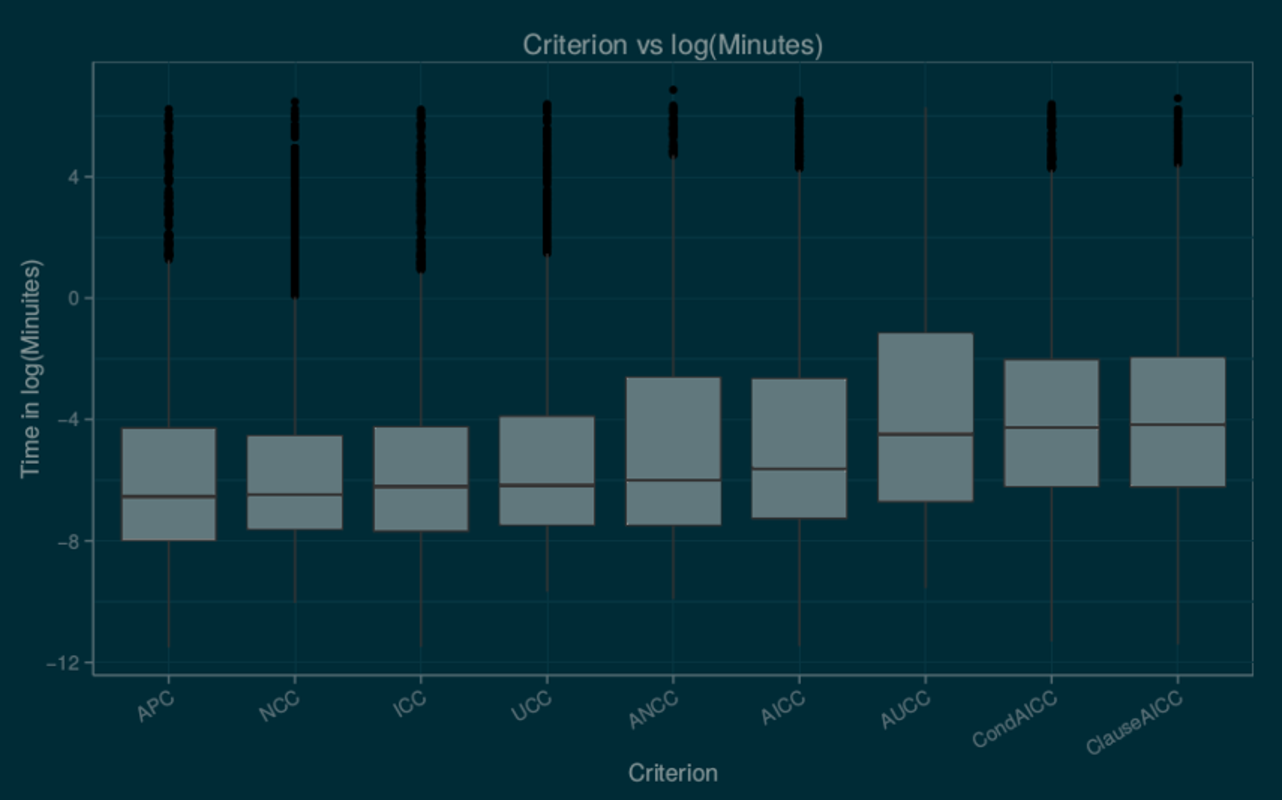
\includegraphics[width=\textwidth]{graphs/CriterionBoxDarker}
  \end{figure}

  \tikzstyle{proc} = [draw, thick, fill=solarizedViolet, text centered, rounded corners,
    text=solarizedRebase02, draw=solarizedViolet]

\tikzstyle{prochighlight} = [draw, thick, fill=solarizedOrange, text centered, rounded corners,
    text=solarizedRebase02, draw=solarizedOrange]

\tikzstyle{procold} = [draw, thick, fill=solarizedViolet!75, text centered, rounded corners,
    text=solarizedRebase02, draw=solarizedViolet!75]

\tikzstyle{procchanged} = [draw, thick, fill=solarizedViolet!75, text centered, rounded corners,
    text=solarizedRebase02, draw=solarizedViolet!75]

\tikzstyle{prochighlightold} = [draw, thick, fill=solarizedOrange!75, text centered, rounded corners,
    text=solarizedRebase02, draw=solarizedOrange!75]

\tikzstyle{prochighlightchanged} = [draw, thick, fill=solarizedYellow!75, text centered, rounded corners,
    text=solarizedRebase02, draw=solarizedYellow!75]

\tikzstyle{proctest} = [draw, thick, fill=solarizedOrange, text centered, rounded corners,
text=solarizedBase02, draw=solarizedOrange]

\tikzstyle{procnew} = [draw, thick, fill=solarizedGreen, text centered, rounded corners,
    text=solarizedRebase02, draw=solarizedGreen]

\tikzstyle{procyellow} = [draw, thick, fill=solarizedYellow, text centered, rounded corners,
    text=solarizedRebase02, draw=solarizedYellow]

\tikzstyle{procred} = [draw, thick, fill=solarizedRed, text centered, rounded corners,
    text=solarizedRebase02, draw=solarizedRed]

\tikzstyle{io} = [ellipse, draw, thick, fill=solarizedBlue, draw=solarizedBlue, text=solarizedRebase02]

\tikzstyle{iopass} = [ellipse, draw, thick, fill=solarizedGreen, draw=solarizedGreen, text=solarizedRebase02]
\tikzstyle{iofail} = [ellipse, draw, thick, fill=solarizedRed, draw=solarizedRed, text=solarizedRebase02]
\tikzstyle{iohighlight} = [ellipse, draw, thick, fill=solarizedYellow, draw=solarizedYellow,
    text=solarizedRebase02]

\tikzstyle{iofailother} = [ellipse, draw, thick, fill=solarizedYellow, draw=solarizedYellow,
    text=solarizedRebase02]
\tikzstyle{wrongoutput} = [ellipse, draw, thick, fill=solarizedCyan, draw=solarizedCyan, text=solarizedRebase02]

\tikzstyle{special} = [draw, thick, fill=solarizedGreen, text centered, draw=solarizedGreen,
    text=solarizedBase02]
\tikzstyle{specialOrange} = [draw, thick, fill=solarizedOrange, text centered, draw=solarizedOrange,
    text=solarizedBase02]
\tikzstyle{specialGreen} = [draw, thick, fill=solarizedGreen, text centered, draw=solarizedGreen,
    text=solarizedBase02]
\tikzstyle{specialYellow} = [draw, thick, fill=solarizedYellow, text centered, draw=solarizedYellow,
    text=solarizedBase02]

\tikzstyle{pass} = [draw, thick, fill=solarizedGreen, text centered, draw=solarizedGreen, text=solarizedRebase02]
\tikzstyle{fail} = [draw, thick, fill=solarizedRed, text centered, draw=solarizedRed, text=solarizedRebase02]

\tikzstyle{feature} = [draw, thick, fill=solarizedOrange, text centered, text=solarizedRebase02, draw=solarizedOrange]

\tikzstyle{plain} = [draw, thick, fill=kapfhammerDarkGrey, text centered, text=solarizedRebase02, draw=kapfhammerDarkGrey]
\tikzstyle{featurecurve} = [draw, thick, fill=solarizedGreen, text centered, rounded corners]

  \vspace{-.075in}

  \begin{figure}
    \begin{centering}
      \begin{tikzpicture}
        \path[use as bounding box] (-5.35,1.5) rectangle (10,-3);
        \path[->]<2-> node[special,]
          (Requirements) at (0,1.75)
          {More effective criteria require additional runtime};
      \end{tikzpicture}
    \end{centering}
  \end{figure}

\end{frame}

\begin{frame}%[label=current]
  \frametitle{Data Generator}
  \framesubtitle{\mbox{}}
  \vspace*{-.1in}
  \begin{figure}
    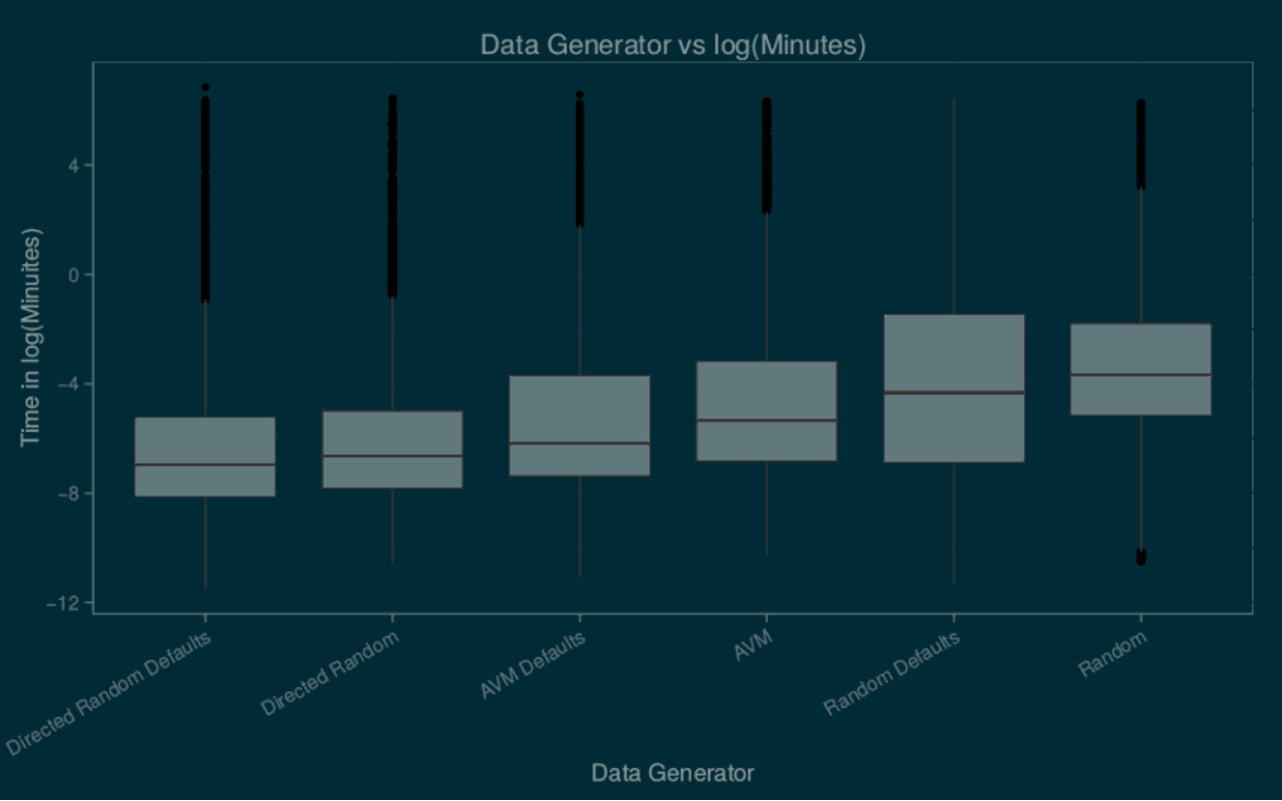
\includegraphics[width=\textwidth]{graphs/DataGeneratorBoxDarker}
  \end{figure}
  \vspace{-.075in}
  \tikzstyle{proc} = [draw, thick, fill=solarizedViolet, text centered, rounded corners,
    text=solarizedRebase02, draw=solarizedViolet]

\tikzstyle{prochighlight} = [draw, thick, fill=solarizedOrange, text centered, rounded corners,
    text=solarizedRebase02, draw=solarizedOrange]

\tikzstyle{procold} = [draw, thick, fill=solarizedViolet!75, text centered, rounded corners,
    text=solarizedRebase02, draw=solarizedViolet!75]

\tikzstyle{procchanged} = [draw, thick, fill=solarizedViolet!75, text centered, rounded corners,
    text=solarizedRebase02, draw=solarizedViolet!75]

\tikzstyle{prochighlightold} = [draw, thick, fill=solarizedOrange!75, text centered, rounded corners,
    text=solarizedRebase02, draw=solarizedOrange!75]

\tikzstyle{prochighlightchanged} = [draw, thick, fill=solarizedYellow!75, text centered, rounded corners,
    text=solarizedRebase02, draw=solarizedYellow!75]

\tikzstyle{proctest} = [draw, thick, fill=solarizedOrange, text centered, rounded corners,
text=solarizedBase02, draw=solarizedOrange]

\tikzstyle{procnew} = [draw, thick, fill=solarizedGreen, text centered, rounded corners,
    text=solarizedRebase02, draw=solarizedGreen]

\tikzstyle{procyellow} = [draw, thick, fill=solarizedYellow, text centered, rounded corners,
    text=solarizedRebase02, draw=solarizedYellow]

\tikzstyle{procred} = [draw, thick, fill=solarizedRed, text centered, rounded corners,
    text=solarizedRebase02, draw=solarizedRed]

\tikzstyle{io} = [ellipse, draw, thick, fill=solarizedBlue, draw=solarizedBlue, text=solarizedRebase02]

\tikzstyle{iopass} = [ellipse, draw, thick, fill=solarizedGreen, draw=solarizedGreen, text=solarizedRebase02]
\tikzstyle{iofail} = [ellipse, draw, thick, fill=solarizedRed, draw=solarizedRed, text=solarizedRebase02]
\tikzstyle{iohighlight} = [ellipse, draw, thick, fill=solarizedYellow, draw=solarizedYellow,
    text=solarizedRebase02]

\tikzstyle{iofailother} = [ellipse, draw, thick, fill=solarizedYellow, draw=solarizedYellow,
    text=solarizedRebase02]
\tikzstyle{wrongoutput} = [ellipse, draw, thick, fill=solarizedCyan, draw=solarizedCyan, text=solarizedRebase02]

\tikzstyle{special} = [draw, thick, fill=solarizedGreen, text centered, draw=solarizedGreen,
    text=solarizedBase02]
\tikzstyle{specialOrange} = [draw, thick, fill=solarizedOrange, text centered, draw=solarizedOrange,
    text=solarizedBase02]
\tikzstyle{specialGreen} = [draw, thick, fill=solarizedGreen, text centered, draw=solarizedGreen,
    text=solarizedBase02]
\tikzstyle{specialYellow} = [draw, thick, fill=solarizedYellow, text centered, draw=solarizedYellow,
    text=solarizedBase02]

\tikzstyle{pass} = [draw, thick, fill=solarizedGreen, text centered, draw=solarizedGreen, text=solarizedRebase02]
\tikzstyle{fail} = [draw, thick, fill=solarizedRed, text centered, draw=solarizedRed, text=solarizedRebase02]

\tikzstyle{feature} = [draw, thick, fill=solarizedOrange, text centered, text=solarizedRebase02, draw=solarizedOrange]

\tikzstyle{plain} = [draw, thick, fill=kapfhammerDarkGrey, text centered, text=solarizedRebase02, draw=kapfhammerDarkGrey]
\tikzstyle{featurecurve} = [draw, thick, fill=solarizedGreen, text centered, rounded corners]

  \begin{figure}
    \begin{centering}
      \begin{tikzpicture}
        \path[use as bounding box] (-5.35,.5) rectangle (10,-3);
        \path[->]<2-> node[special,]
          (Requirements) at (0,.75)
          {More effective generators can also be more efficient};
      \end{tikzpicture}
    \end{centering}
  \end{figure}
\end{frame}


\section{Conclusion}
\tikzstyle{proc} = [draw, thick, fill=solarizedViolet, text centered, rounded corners,
    text=solarizedRebase02, draw=solarizedViolet]

\tikzstyle{prochighlight} = [draw, thick, fill=solarizedOrange, text centered, rounded corners,
    text=solarizedRebase02, draw=solarizedOrange]

\tikzstyle{procold} = [draw, thick, fill=solarizedViolet!75, text centered, rounded corners,
    text=solarizedRebase02, draw=solarizedViolet!75]

\tikzstyle{procchanged} = [draw, thick, fill=solarizedViolet!75, text centered, rounded corners,
    text=solarizedRebase02, draw=solarizedViolet!75]

\tikzstyle{prochighlightold} = [draw, thick, fill=solarizedOrange!75, text centered, rounded corners,
    text=solarizedRebase02, draw=solarizedOrange!75]

\tikzstyle{prochighlightchanged} = [draw, thick, fill=solarizedYellow!75, text centered, rounded corners,
    text=solarizedRebase02, draw=solarizedYellow!75]

\tikzstyle{proctest} = [draw, thick, fill=solarizedOrange, text centered, rounded corners,
text=solarizedBase02, draw=solarizedOrange]

\tikzstyle{procnew} = [draw, thick, fill=solarizedGreen, text centered, rounded corners,
    text=solarizedRebase02, draw=solarizedGreen]

\tikzstyle{procyellow} = [draw, thick, fill=solarizedYellow, text centered, rounded corners,
    text=solarizedRebase02, draw=solarizedYellow]

\tikzstyle{procred} = [draw, thick, fill=solarizedRed, text centered, rounded corners,
    text=solarizedRebase02, draw=solarizedRed]

\tikzstyle{io} = [ellipse, draw, thick, fill=solarizedBlue, draw=solarizedBlue, text=solarizedRebase02]

\tikzstyle{iopass} = [ellipse, draw, thick, fill=solarizedGreen, draw=solarizedGreen, text=solarizedRebase02]
\tikzstyle{iofail} = [ellipse, draw, thick, fill=solarizedRed, draw=solarizedRed, text=solarizedRebase02]
\tikzstyle{iohighlight} = [ellipse, draw, thick, fill=solarizedYellow, draw=solarizedYellow,
    text=solarizedRebase02]

\tikzstyle{iofailother} = [ellipse, draw, thick, fill=solarizedYellow, draw=solarizedYellow,
    text=solarizedRebase02]
\tikzstyle{wrongoutput} = [ellipse, draw, thick, fill=solarizedCyan, draw=solarizedCyan, text=solarizedRebase02]

\tikzstyle{special} = [draw, thick, fill=solarizedGreen, text centered, draw=solarizedGreen,
    text=solarizedBase02]
\tikzstyle{specialOrange} = [draw, thick, fill=solarizedOrange, text centered, draw=solarizedOrange,
    text=solarizedBase02]
\tikzstyle{specialGreen} = [draw, thick, fill=solarizedGreen, text centered, draw=solarizedGreen,
    text=solarizedBase02]
\tikzstyle{specialYellow} = [draw, thick, fill=solarizedYellow, text centered, draw=solarizedYellow,
    text=solarizedBase02]

\tikzstyle{pass} = [draw, thick, fill=solarizedGreen, text centered, draw=solarizedGreen, text=solarizedRebase02]
\tikzstyle{fail} = [draw, thick, fill=solarizedRed, text centered, draw=solarizedRed, text=solarizedRebase02]

\tikzstyle{feature} = [draw, thick, fill=solarizedOrange, text centered, text=solarizedRebase02, draw=solarizedOrange]

\tikzstyle{plain} = [draw, thick, fill=kapfhammerDarkGrey, text centered, text=solarizedRebase02, draw=kapfhammerDarkGrey]
\tikzstyle{featurecurve} = [draw, thick, fill=solarizedGreen, text centered, rounded corners]

\begin{frame}[t]{Important Contributions}

  \hspace*{-.5in}
  \begin{minipage}{5in}
  \begin{center}

    \begin{minipage}{4.5in}

    % Derby.png
    \pgfdeclareimage[height=4ex]{Derby}{Derby.png}
    
    % HSQLDB.png
    \pgfdeclareimage[height=4ex]{Hsqldb}{HSQLDB.png}

    % IBMDB2.png
    \pgfdeclareimage[height=4ex]{Db2}{IBMDB2.png}
    
    % MySQL.png
    \pgfdeclareimage[height=4ex]{My}{mysql-logo-1.jpg}

    % Postgres.png
    \pgfdeclareimage[height=10ex]{Postgres}{logo_w_elephant.pdf}

    % SQLite.png
    \pgfdeclareimage[height=4ex]{Sqlite}{SQLite.png}    

    \begin{figure}

    \begin{center}

      \begin{tikzpicture}[node distance=1cm, auto,>=stealth, thick]
	
        \path[use as bounding box] (-2,3.5) rectangle (10,-2);

      	\path[->]<1-> node[prochighlight, text width=54ex] 
        (Loss) at (4,2.8) 
        {This paper introduces a framework that empirically
determines  an  algorithm’s  worst-case  time  complexity  by
doubling the size of the input and observing the change in
runtime.};

        \path[->]<2-> node[proc, below of=Loss, text width=48ex,
          yshift=-.225in, xshift=0in] (Comment) {Empirically derived suggestions
            for the worst-case time complexity of search-based test data generators.};

        \path[->]<3-> node[proc, below of=Comment, text width=48ex,
          yshift=-.1in, xshift=0in] (CommentAgain) {With a systematic focus on a wide
            variety of configurations, an empirical study revealing trade-offs in search-
            based test data generation for relational schemas.};

        \path[->]<4-> node[proc, below of=CommentAgain, text
          width=48ex, yshift=-.1in, xshift=0in] (CommentOneMore) {{\em
            SchemaAnalyst}'s mutation score is higher than {\em
            DBMonster}'s for 96\% of the schemas};

        \path[->]<5-> node[prochighlight, below of=CommentOneMore, text
          width=36ex, yshift=-.025in, xshift=0in] (CommentFinal) 
        {https://github.com/kinneerc/ExpOse};

        %% \path[->]<3-> node[prochighlight, below of=Ambler, text width=48ex,
        %%   yshift=-.5in, xshift=0in] (SchemaAnalyst) 
        %% {This paper presents {\em SchemaAnalyst}, a search-based
        %%   system for testing the complex \\ integrity constraints in
        %%   relational schemas};

 	\end{tikzpicture}
	
        \end{center}

        \end{figure}
      
      \end{minipage} 

  \end{center}
  \end{minipage}

\end{frame}



\end{document}
